\documentclass{article}

%\usepackage[T1]{fontenc}
%\usepackage[utf8]{inputenc}

\usepackage{enumerate}

\usepackage{stix}
\usepackage{amsmath,amsfonts,mathtools,stackrel}
%\setlength{\mathindent}{0pt}
\allowdisplaybreaks

\usepackage{amsthm}
\newtheorem{theorem}{Theorem}
\newtheorem{definition}[theorem]{Definition}
\newtheorem{lemma}[theorem]{Lemma}
\newtheorem{corollary}[theorem]{Corollary}

\usepackage{breqn}

\usepackage{listings}
\lstset{mathescape=true}
\newcommand{\lst}[1]{\lstinline!#1!}

\usepackage{bcprules}

\usepackage{tikz,tikz-cd}
\tikzset{%
  symbol/.style={%
    draw=none,
    every to/.append style={%
      edge node={node [sloped, allow upside down, auto=false]{$#1$}}}
  }
}

% custom macros
\newcommand{\minus}{{\scalebox{0.9}{-}}}
\newcommand{\plus}{{\scalebox{0.6}{\!+}}}
\newcommand{\squarediamond}{\mathbin{\text{\tikz [x=1ex,y=1ex,scale=1.5,line width=.1ex,line join=round] \draw (0,0) rectangle (1,1) (.5\pgflinewidth,.5) -- (.5,1ex-.5\pgflinewidth) -- (1ex-.5\pgflinewidth,.5) -- (.5,.5\pgflinewidth) -- (.5\pgflinewidth,.5) -- cycle;}}}
\renewcommand{\square}{\mathbin{\text{\tikz [x=1ex,y=1ex,scale=1.5,line width=.1ex,line join=round] \draw (0,0) rectangle (1,1);}}}
\renewcommand{\diamond}{\mathbin{\text{\tikz [x=1ex,y=1ex,scale=1.5,line width=.1ex,line join=round] \draw (.5\pgflinewidth,.5) -- (.5,1ex-.5\pgflinewidth) -- (1ex-.5\pgflinewidth,.5) -- (.5,.5\pgflinewidth) -- (.5\pgflinewidth,.5) -- cycle;}}}
\newcommand{\state}[1]{\ensuremath \langle #1 \rangle}
\newcommand{\transition}[2]{\ensuremath \state{#1} & \longrightarrow \state{#2}}
\newcommand{\termrule}[3]{\ensuremath #1 \xrightarrow{#2} #3}
\newcommand{\fail}{\ensuremath \text{$\uparrow$}}
\newcommand{\success}{\ensuremath \text{$\downarrow$}}
\newcommand{\cont}[2]{\ensuremath \mathbf{#1}(#2)}
\newcommand{\return}{\ensuremath \hookleftarrow}
\newcommand{\seq}[2]{\ensuremath #1 ; #2}
\newcommand{\choice}[2]{\ensuremath #1 + #2}
\newcommand{\leftchoice}[2]{\ensuremath #1 \mathrel{\vcenter{\hbox{+}}\mkern-18.5mu{\leftarrow}} #2}
\newcommand{\fix}[2]{\ensuremath \operatorname{rec}(#1,#2)}
\newcommand{\path}[2]{\ensuremath \operatorname{path}(#1,#2)}
\newcommand{\one}[1]{\ensuremath \operatorname{one}(#1)}
\newcommand{\all}[1]{\ensuremath \operatorname{all}(#1)}
\newcommand{\some}[1]{\ensuremath \operatorname{some}(#1)}
\newcommand{\congr}[1]{\ensuremath \operatorname{cong}(#1)}
\newcommand{\match}[1]{\ensuremath \operatorname{match}(#1)}
\newcommand{\build}[1]{\ensuremath \operatorname{build}(#1)}
\newcommand{\where}[1]{\ensuremath \operatorname{where}(#1)}
\newcommand{\test}[1]{\ensuremath \operatorname{test}(#1)}
\newcommand{\scope}[2]{\ensuremath \lbrace #1 : #2 \rbrace}
\newcommand{\vars}[1]{\ensuremath \text{vars}(#1)}
\newcommand{\alt}{\ensuremath \; | \;}
\newcommand{\subst}[3]{\ensuremath #1[#2 / #3]}

\newcommand{\transform}[5]{#1, #2 \xrightarrow{#3} #4, #5}
\newcommand{\transformx}[4]{#1, #2 \xrightarrow{#3} #4}
\newcommand{\transformfail}[3]{#1, #2 \xrightarrow{#3} \fail}
\newcommand{\dom}[1]{\ensuremath \text{dom}(#1)}
\newcommand{\cjm}{\ensuremath \xmapsto{\text{\tiny cjm}}}
\newcommand{\mon}{\ensuremath \xmapsto{\text{\tiny mon}}}

\newcommand{\Term}{\ensuremath \mathbb{T}}
\newcommand{\Fail}{\ensuremath \mathbb{F}}
\newcommand{\Var}{\ensuremath \mathbb{V}}
\newcommand{\Constructors}{\ensuremath \mathcal{Con}}
\newcommand{\Env}{\ensuremath \Var \mapsto \Term}
\newcommand{\Pow}[1]{\ensuremath \mathcal{P}(#1)}
\newcommand{\sem}[1]{\ensuremath \lBrack* #1 \rBrack*}

\newcommand{\State}{\ensuremath \text{State}}
\newcommand{\Statea}{\ensuremath \widehat{\State}}

\newcommand{\setbuild}[2]{\ensuremath \left\{\, #1 \mid #2 \,\right\}}
\newcommand{\setbuildc}[1]{\ensuremath \left\{\, #1 \,\right\}}

\newcommand{\id}{\ensuremath \operatorname{id}}
\newcommand{\Rel}{\ensuremath \mathbf{Rel}}
\newcommand{\Naive}{\ensuremath \mathbf{Naive}}
\newcommand{\adjoint}{\ensuremath \dashv}
\newcommand{\lub}{\ensuremath \bigsqcup}
\newcommand{\glb}{\ensuremath \bigsqcap}

\newcommand{\Salgebra}{\ensuremath \mathcal{S}\text{-algebra}}
\newcommand{\Salgebras}{\ensuremath \mathcal{S}\text{-algebras}}
\newcommand{\Salg}{\ensuremath \mathcal{S}}
\newcommand{\lfail}{\ensuremath \operatorname{fail}}
\newcommand{\lsucc}{\ensuremath \operatorname{succ}}
\newcommand{\set}{\ensuremath \operatorname{set}}
\newcommand{\get}{\ensuremath \operatorname{get}}
\newcommand{\arity}{\ensuremath \operatorname{arity}}
\newcommand{\constructor}{\ensuremath \operatorname{con}}

\begin{document}

\section{Abstract Interpretation of System S}

\begin{definition}[Operational semantics of System S] \normalfont
\end{definition}

\infrule[Test]
  {\transform{t}{\rho}{s}{t'}{\rho'}}
  {\transform{t}{\rho}{\test{s}}{t}{\rho}}

\infrule[Test-Fail]
  {\transformfail{t}{\rho}{s}}
  {\transformfail{t}{\rho}{\test{s}}}

\infrule[Neg]
  {\transformfail{t}{\rho}{s}}
  {\transform{t}{\rho}{\neg s}{t}{\rho}}

\infrule[Neg-Fail]
  {\transform{t}{\rho}{s}{t'}{\rho'}}
  {\transformfail{t}{\rho}{\neg s}}

\infrule[Seq]
  {\transform{t}{\rho}{s_1}{t'}{\rho'} \andalso \transform{t'}{\rho'}{s_2}{t''}{\rho''}}
  {\transform{t}{\rho}{\seq{s_1}{s_2}}{t''}{\rho''}}

\infrule[Seq-Fail-1]
  {\transformfail{t}{\rho}{s_1}}
  {\transformfail{t}{\rho}{\seq{s_1}{s_2}}}

\infrule[Seq-Fail-2]
  {\transform{t}{\rho}{s_1}{t'}{\rho'} \andalso \transformfail{t'}{\rho'}{s_2}}
  {\transformfail{t}{\rho}{\seq{s_1}{s_2}}}

\infrule[Choice-1]
  {\transform{t}{\rho}{s_1}{t'}{\rho'}}
  {\transform{t}{\rho}{\choice{s_1}{s_2}}{t'}{\rho'}}

\infrule[Choice-2]
  {\transform{t}{\rho}{s_2}{t'}{\rho'}}
  {\transform{t}{\rho}{\choice{s_1}{s_2}}{t'}{\rho'}}

\infrule[Choice-Fail]
  {\transformfail{t}{\rho}{s_1} \andalso \transformfail{t}{\rho}{s_2}}
  {\transformfail{t}{\rho}{\choice{s_1}{s_2}}}

\infrule[Left-Choice-1]
  {\transform{t}{\rho}{s_1}{t'}{\rho'}}
  {\transform{t}{\rho}{\leftchoice{s_1}{s_2}}{t'}{\rho'}}

\infrule[Left-Choice-2]
  {\transformfail{t}{\rho}{s_1} \andalso \transform{t}{\rho}{s_2}{t'}{\rho'}}
  {\transform{t}{\rho}{\leftchoice{s_1}{s_2}}{t'}{\rho'}}

\infrule[Left-Choice-Fail]
  {\transformfail{t}{\rho}{s_1} \andalso \transformfail{t}{\rho}{s_2}}
  {\transformfail{t}{\rho}{\choice{s_1}{s_2}}}

\infrule[Rec]
  {\transform{t}{\rho}{\subst{s}{x}{\fix{x}{s}}}{t'}{\rho'}}
  {\transform{t}{\rho}{\fix{x}{s}}{t'}{\rho'}}

\infrule[Rec-Fail]
  {\transformfail{t}{\rho}{\subst{s}{x}{\fix{x}{s}}}}
  {\transformfail{t}{\rho}{\fix{x}{s}}}

\infrule[Path]
  {\transform{t_i}{\rho}{s}{t_i'}{\rho'}}
  {\transform{f(\ldots,t_i,\ldots)}{\rho}{\path{i}{s}}{f(\ldots,t_i',\ldots)}{\rho'}}

\infrule[Path-Fail]
  {\transformfail{t_i}{\rho}{s}}
  {\transformfail{f(\ldots,t_i,\ldots)}{\rho}{\path{i}{s}}}

\infrule[Path-Fail-Bounds]
  {i > n}
  {\transformfail{f(t_1,\ldots,t_n)}{\rho}{\path{i}{s}}}

\infrule[Cong]
  {\transform{t_i}{\rho_i}{s_i}{t_i'}{\rho_{i+1}} \text{ for all } 1 \leq i \leq n}
  {\transform{f(t_1,\ldots,t_n)}{\rho_1}{\congr{f,s_1,\ldots,s_n}}{f(t_1',\ldots,t_n')}{\rho_{n+1}}}

\infrule[Cong-Fail]
  {\transform{t_i}{\rho_i}{s_i}{t_i'}{\rho_{i+1}} \text{ for all } 1 \leq i < k \andalso \transformfail{t_k}{\rho_k}{s_k} \andalso k \leq n}
  {\transformfail{f(t_1,\ldots,t_n)}{\rho_1}{\congr{f,s_1,\ldots,s_n}}}

\infrule[Cong-Con-Fail]
  {f \neq g}
  {\transformfail{f(t_1,\ldots,t_n)}{\rho}{\congr{g,t_1',\ldots,t_n'}}}

\infrule[Cong-Arity-Fail]
  {n \neq n'}
  {\transformfail{f(t_1,\ldots,t_n)}{\rho}{\congr{g,t_1',\ldots,t_{n'}'}}}

\infrule[One]
  {\transform{t_i}{\rho}{s}{t_i'}{\rho'}}
  {\transform{f(\ldots,t_i,\ldots)}{\rho}{\one{s}}{f(\ldots,t_i',\ldots)}{\rho'}}

\infrule[One-Fail]
  {\transformfail{t_1}{\rho}{s} \andalso \cdots \andalso \transformfail{t_n}{\rho}{s}}
  {\transformfail{f(t_1,\ldots,t_n)}{\rho}{\one{s}}}

\infrule[All]
  {\transform{t_i}{\rho_i}{s}{t_i'}{\rho_{i+1}} \text{ for all } 1 \leq i \leq n}
  {\transform{f(t_1,\ldots,t_n)}{\rho_1}{\all{s}}{f(t_1',\ldots,t_n')}{\rho_{n+1}}}

\infrule[All-Fail]
  {\transform{t_i}{\rho_i}{s}{t_i'}{\rho_{i+1}} \text{ for all } 1 \leq i < k \andalso \transformfail{t_k}{\rho_k}{s_k} \andalso k \leq n}
  {\transformfail{f(t_1,\ldots,t_n)}{\rho_1}{\all{s}}}

\infrule[Some]
  {\transform{t_i}{\rho_i}{s}{t_i'}{\rho_{i+1}} \text{ for all } i \in M \\
   \transformfail{t_j}{\rho_j}{s} \land\ \rho_{j+1} = \rho_j \land t_j' = t_j \text{ for all } j \in \overline{M} \\
   M \subseteq \lbrace 1 \ldots n \rbrace}
  {\transform{f(t_1,\ldots,t_n)}{\rho_1}{\some{s}}{f(t_1',\ldots,t_n')}{\rho_{n+1}}}

\infrule[Some-Fail]
  {\transformfail{t_i}{\rho}{s} \text{ for all } 1 \leq i \leq n}
  {\transformfail{f(t_1,\ldots,t_n)}{\rho}{\some{s}}}

\infrule[Match-Not-In-Dom]
  {x \notin \dom{\rho}}
  {\transform{t}{\rho}{\match{x}}{t}{\rho[x \mapsto t]}}

\infrule[Match-In-Dom]
  {\rho(x) = t}
  {\transform{t}{\rho}{\match{x}}{t}{\rho}}

\infrule[Match-In-Dom-Fail]
  {\rho(x) \neq t}
  {\transformfail{t}{\rho}{\match{x}}}

\infrule[Match-Sub]
  {\transform{t_i}{\rho_i}{\match{t_i'}}{t_i}{\rho_{i+1}} \text{ for all } 1 \leq i \leq n}
  {\transform{f(t_1,\ldots,t_n)}{\rho_1}{\match{f(t_1',\ldots,t_n')}}{f(t_1,\ldots,t_n)}{\rho_n}}

\infrule[Match-Sub-Fail]
  {\transform{t_i}{\rho_i}{\match{t_i'}}{t_i}{\rho_{i+1}} \text{ for all } 1 \leq i < k \\
   \transformfail{t_k}{\rho_k}{\match{t_k'}} \\
   k \leq n}
  {\transform{f(t_1,\ldots,t_n)}{\rho_1}{\match{f(t_1',\ldots,t_n')}}{f(t_1,\ldots,t_n)}{\rho_n}}

\infrule[Match-Con-Fail]
  {f \neq g}
  {\transformfail{f(t_1,\ldots,t_n)}{\rho}{\match{g(t_1',\ldots,t_n')}}}

\infrule[Build]
  {\vars{t'} \subseteq \dom{\rho}}
  {\transform{t}{\rho}{\build{t'}}{\rho(t')}{\rho}}

\infrule[Build-Fail]
  {\vars{t'} \nsubseteq \dom{\rho}}
  {\transformfail{t}{\rho}{\build{t'}}}

\infrule[Where]
  {\transform{t}{\rho}{s}{\rho(t')}{\rho'}}
  {\transform{t}{\rho}{\where{s}}{t}{\rho'}}

\infrule[Where-Fail]
  {\transformfail{t}{\rho}{s}}
  {\transformfail{t}{\rho}{\where{s}}}

\infrule[Scope]
  {\transform{t}{\rho \setminus \mathbf{x}}{s}{t'}{\rho'}}
  {\transform{t}{\rho}{\scope{\mathbf{x}}{s}}{t'}{(\rho' \setminus \mathbf{x}) \cup (\rho | \mathbf{x})}}

\infrule[Scope-Fail]
  {\transformfail{t}{\rho \setminus \mathbf{x}}{s}}
  {\transformfail{t}{\rho}{\scope{\mathbf{x}}{s}}}

\par\medskip

\begin{definition}[$\Rel$ Category] \normalfont
  We define the category of relations $\Rel$, with sets $A,B,C, \ldots$ as objects, binary relation $R,S,T, \ldots$ as arrows where $R: A \rightarrow B$ if $R \subseteq A \times B,$ identity arrows \[\id_A \coloneqq \setbuild{ (x,x) }{ x \in A },\] composition of relations \[R \circ S \coloneqq \setbuild{(x,z)}{ \exists y. (x,y) \in S \land (y,z) \in R }.\] Additionally, for all relations $R \subseteq A \times B$ there is a symmetric relation $R^{-1} \subseteq B \times A$ defined as \[ R^{-1} \coloneqq \setbuild{(y,x)}{ \forall (x,y) \in R }, \] Notice however that $R^{-1} \circ R$ is not necessarily equal to $\id$.
\end{definition}

\begin{definition}[$\Rel(A)$ Category] \normalfont
  We define the category $\Rel(A)$ as a proper subcategory of $\Rel$, where the all the objects are subsets of $A$.
\end{definition}

\begin{definition}[System S Programm State] \normalfont
  We define the state space of System S programs as \[\State \coloneqq \Term \times \Env \cup \Fail,\] the set of all terms together with a term environment or failure.
\end{definition}

We can think of the category $\Rel(\State)$ as a category with properties of program states as objects and relations between two program states as arrows.

\begin{definition}[$\Salgebra$] \normalfont
  An $\Salgebra$, is an abstract algebra to represent operations for term rewriting. The algebra consists of
  \begin{itemize}
    \item a partially ordered set $A$ equipped with for all $a, a_1, a_2 \in A$,
    \item binary \emph{meet} $a_1 \sqcap a_2$ and \emph{join} $a_1 \sqcup a_2$ operations,
    \item an unary \emph{reverse} operation $a^{-1}$,
    \item constant symbols to represent success ($\lsucc_a$) and failure ($\lfail_a$) of a strategy,
    \item an unary operation to retrieve the $i$th immediate subterm ($\get_a(i)$),
    \item two unary operations that assert if the top most constructor is equal $(\constructor = f)_a$ or not equal $(\constructor \neq f)_a$ to another constructor symbol $f$,
    \item two unary operations that assert if the arity of the top level constructor is lower $(\arity < i)_a$ or greater $(i < \arity)_a$ than a number $i$.
  \end{itemize}
  When it is clear from the context, we omit the subscripts of the operations. We refer with $\Salg(A)$ to an $\Salgebra$ with the underlying set $A$.

  \par\medskip
   
  A morphism between two $\Salgebras$ $\Salg(A)$ and $\Salg(B)$ is a galois connection 
  \[
    \begin{tikzcd}
      A\ar[r,bend left,"\alpha",""{name=A, below}] & B\ar[l,bend left,"\gamma",""{name=B,above}] \ar[from=A, to=B, symbol=\dashv]
    \end{tikzcd},
  \] where $\alpha$ preserves the algebraic operations of the $\Salgebras$ up to sound over approximation, that is, for all $a,a_1, a_2 \in A, i \in \mathbb{N}, f \in \Constructors$,
  \begin{align*}
    \alpha(a_1 \sqcap a_2) &\leq \alpha(a_1) \sqcap \alpha(a_1) \\
    \alpha(a_1 \sqcup a_2) &\leq \alpha(a_1) \sqcup \alpha(a_1) \\
    \alpha(\lsucc_a)       &\leq \lsucc_{\alpha(a)} \\
    \alpha(\lfail_a)       &\leq \lfail_{\alpha(a)} \\
    \alpha(\get_a(i))       &\leq \get_{\alpha(a)}(i) \\
  \end{align*}
  We say, that the morphism is strict, when $\alpha$ preserves the algebraic operations up to equality.
  
  \begin{itemize}
    \item binary \emph{meet} $\sqcap$ and \emph{join} $\sqcup$ operations,
    \item an unary \emph{reverse} operation $(-)^{-1}$,
    \item constant symbols to represent success ($\lsucc$) and failure ($\lfail$) of a strategy,
    \item an unary operation to retrieve the $i$th immediate subterm ($\get(i)$),
    \item two unary operations to assert if the top most constructor is equal $(\constructor = -)$ or not equal $(\constructor \neq -)$ to another constructor symbol,
    \item two unary operations to assert if the arity of the top level constructor is lower $(\arity < -)$ or greater $(- < \arity)$ than a certain number.
  \end{itemize}
\end{definition}

\begin{definition}[$\Salgebra$ for $\Rel(\State)$] \normalfont
  We define an $\Salgebra$ for binary relations over System S states, with 
  \begin{itemize}
    \item $L = \State \times \State$,
    \item for two relations $R : A_1 \rightarrow A_2$ and $S : B_1 \rightarrow B_2$ the meet operation $R \sqcap S : A_1 \cap B_1 \rightarrow A_2 \cap B_2$ as the intersection of relations defined by \[R \sqcap S \coloneqq R \cap S, \] and join $R \sqcup S : A_1 \cup B_1 \rightarrow A_2 \cup B_2$ as the union of relations defined by \[ R \sqcup S \coloneqq R \cup S, \]
    \item the reverse operation $(-)^{-1}$ as defined in $\Rel(\State)$,
    \item for all objects $A$, the \emph{success} operation as an morphism defined by \[\lsucc \coloneqq \setbuild{((t,\rho),(t,\rho))}{ \forall (t,\rho) \in A }, \]
    \item for all objects $A$, the \emph{failure} operation as an morphism defined by \[ \lfail \coloneqq \setbuild{((t,\rho),\fail)}{ \forall (t,\rho) \in A }, \]
    \item for all objects $A$, the retrieval operation of the $i$th immediate subterm as an morphism defined by \[ \get(i) \coloneqq \setbuild{ ((f(\ldots t_i \ldots),\rho), (t_i,\rho)) }{ \forall (f(\ldots),\rho) \in A }, \]
    \item for all objects $A$, the assertion of top most constructors as an morphism defined by \[ (\constructor = f) \coloneqq \setbuild{ ((g(\ldots),\rho),(g(\ldots),\rho)) }{ \forall (g(\ldots),\rho) \in A.\ f = g } \] and \[ (\constructor \neq f) \coloneqq \setbuild{ ((g(\ldots),\rho),(g(\ldots),\rho)) }{ \forall (g(\ldots),\rho) \in A.\ f \neq g }, \]
    \item for all objects $A$, the assertion operations of the arity of the top most constructor as morphisms defined by \[ (\arity < i) \coloneqq \setbuild{ ((f(\ldots t_k),\rho),(f(\ldots t_k),\rho)) }{ \forall (f(\ldots t_k),\rho) \in A.\ k < i }, \] and \[ (i < \arity) \coloneqq \setbuild{ ((f(\ldots t_j),\rho),(f(\ldots t_j),\rho)) }{ \forall (f(\ldots t_k),\rho) \in A.\ i < j }, \]
  \end{itemize}

  For convenience, we define notation for replacing the $i$th immediate subterm  
  \[ \set(i) \coloneqq \get(i)^{-1}, \] and asserting if the arity of the top most constructor is not equal to a certain number \[ (\arity \neq i) \coloneqq (\arity < i) \cup (i < \arity). \]
\end{definition}

\begin{definition}[Concrete Denotational Semantics of System S] \normalfont
  We define the denotational semantics of System S programs as a relation over $\State \times \State$ with \[\sem{s} \coloneqq \setbuild{((t,\rho),x)}{\transformx{t}{\rho}{s}{x}}.\]
\end{definition}

\begin{theorem} \normalfont
  Next, we demonstrate that the concrete semantics of System S can be expressed with a $\Salgebra$. We continue by structural induction on System S programs.
\begin{proof}
\begin{dgroup*}
\begin{dmath*}
  \sem{\test{s}}
     = {\setbuild{((t,\rho),x)}{\transformx{t}{\rho}{\test{s}}{x}}}
     = {\setbuild{((t,\rho),(t,\rho))}{\transform{t}{\rho}{s}{t'}{\rho'}}} \cup
       {\setbuild{((t,\rho),\fail)}{\transformfail{t}{\rho}{s}}}
     = \left({\setbuild{((t,\rho),(t,\rho))}{\forall t,\rho}} \circ
             {\setbuild{((t,\rho),x)}{\transformx{t}{\rho}{s}{x}}}\right)^{-1} \circ
       \left({\setbuild{((t,\rho),(t,\rho))}{\forall t,\rho}} \circ
             {\setbuild{((t,\rho),x)}{\transformx{t}{\rho}{s}{x}}}\right) \cup
       {\setbuild{((t,\rho),\fail)}{\forall t, \rho}} \circ
       {\setbuild{((t,\rho),x)}{\transformx{t}{\rho}{s}{x}}}
     = (\lsucc \circ \sem{s})^{-1} \circ (\lsucc \circ \sem{s}) \sqcup \lfail \circ \sem{s}
\end{dmath*}
     
\begin{dmath*}
  \sem{\neg{s}}
    = {\setbuild{((t,\rho),x)}{\transformx{t}{\rho}{\neg{s}}{x}}}
    = {\setbuild{((t,\rho),(t,\rho))}{\transformfail{t}{\rho}{s}}} \cup
      {\setbuild{((t,\rho),\fail)}{\transform{t}{\rho}{s}{t'}{\rho'}}}
    = \left({\setbuild{((t,\rho),\fail)}{\forall t,\rho}} \circ
            {\setbuild{((t,\rho),x)}{\transformx{t}{\rho}{s}{x}}}\right)^{-1} \circ
      \left({\setbuild{((t,\rho),\fail)}{\forall t,\rho}} \circ
            {\setbuild{((t,\rho),x)}{\transformx{t}{\rho}{s}{x}}}\right) \cup
      {\setbuild{((t,\rho),\fail)}{\forall t, \rho}} \circ
      {\setbuild{((t,\rho),(t,\rho))}{\forall t, \rho}} \circ
      {\setbuild{((t,\rho),x)}{\transformx{t}{\rho}{s}{x}}}
    = (\lfail \circ \sem{s})^{-1} \circ (\lfail \circ \sem{s}) \sqcup
       \lfail \circ \lsucc \circ \sem{s}
\end{dmath*}

\begin{dmath*}
  \sem{\seq{s_1}{s_2}}
    = {\setbuild{((t,\rho),x)}{\transformx{t}{\rho}{\seq{s_1}{s_2}}{x}}}
    = {\setbuild{((t,\rho),(t'',\rho''))}{\transform{t}{\rho}{s_1}{t'}{\rho'} \land \transform{t'}{\rho'}{s_2}{t''}{\rho''}}} \cup
      {\setbuild{((t,\rho),\fail)}{\transformfail{t}{\rho}{s_1}}} \cup
      {\setbuild{((t,\rho),\fail)}{\transform{t}{\rho}{s_1}{t'}{\rho'} \land \transformfail{t'}{\rho'}{s_2}}}
    = {\setbuild{((t,\rho),x)}{\transform{t}{\rho}{s_1}{t'}{\rho'} \land \transformx{t'}{\rho'}{s_2}{x}}} \cup
      {\setbuild{((t,\rho),\fail)}{\transformfail{t}{\rho}{s_1}}}
    = {\setbuild{((t,\rho),x)}{\transformx{t'}{\rho'}{s_2}{x}}} \circ
      {\setbuild{((t,\rho),x)}{\transformx{t'}{\rho'}{s_1}{x}}} \cup
      {\setbuild{((t,\rho),\fail)}{\transformfail{t}{\rho}{s_1}}}
    = \sem{s_2} \circ \sem{s_1} \sqcup \lfail \circ \sem{s_1}
\end{dmath*}

\begin{dmath*}
  \sem{\choice{s_1}{s_2}}
     = {\setbuild{((t,\rho),x)}{\transformx{t}{\rho}{\choice{s_1}{s_2}}{x}}}
     = {\setbuild{((t,\rho),(t',\rho'))}{\transform{t}{\rho}{s_1}{t'}{\rho'}}} \cup
       {\setbuild{((t,\rho),(t',\rho'))}{\transform{t}{\rho}{s_2}{t'}{\rho'}}} \cup
       {\setbuild{((t,\rho),\fail)}{\transformfail{t}{\rho}{s_1} \land \transformfail{t'}{\rho'}{s_2}}}
     = {\setbuild{((t,\rho),(t,\rho))}{\forall t, \rho}} \circ
       {\setbuild{((t,\rho),x)}{\transformx{t}{\rho}{s_1}{x}}} \cup
       {\setbuild{((t,\rho),(t,\rho))}{\forall t, \rho}} \circ
       {\setbuild{((t,\rho),x)}{\transformx{t}{\rho}{s_2}{x}}} \cup
       \left({\setbuild{((t,\rho),\fail)}{\forall t, \rho}} \circ
             {\setbuild{((t,\rho),x)}{\transformx{t}{\rho}{s_1}{x}}} \cap
             {\setbuild{((t,\rho),\fail)}{\forall t, \rho}} \circ
             {\setbuild{((t,\rho),x)}{\transformx{t}{\rho}{s_2}{x}}} \right)
     = \lsucc \circ \sem{s_1} \sqcup \lsucc \circ \sem{s_2} \sqcup (\lfail \circ \sem{s_1} \sqcap \lfail \circ \sem{s_2})
\end{dmath*}

\begin{dmath*}
  \sem{\leftchoice{s_1}{s_2}}
     = {\setbuild{((t,\rho),x)}{\transformx{t}{\rho}{\leftchoice{s_1}{s_2}}{x}}}
     = {\setbuild{((t,\rho),(t',\rho'))}{\transform{t}{\rho}{s_1}{t'}{\rho'}}} \cup
       {\setbuild{((t,\rho),(t',\rho'))}{\transformfail{t}{\rho}{s_1} \land \transform{t}{\rho}{s_2}{t'}{\rho'}}} \cup
       {\setbuild{((t,\rho),\fail)}{\transformfail{t}{\rho}{s_1} \land \transformfail{t'}{\rho'}{s_2}}}
     = {\setbuild{((t,\rho),(t',\rho'))}{\transform{t}{\rho}{s_1}{t'}{\rho'}}} \cup
       {\setbuild{((t,\rho),x)}{\transformfail{t}{\rho}{s_1} \land \transformx{t}{\rho}{s_2}{x}}}
     = {\setbuild{((t,\rho),(t,\rho))}{\forall t, \rho}} \circ
       {\setbuild{((t,\rho),x)}{\transformx{t}{\rho}{s_1}{x}}} \cup
       {\setbuild{((t,\rho),x)}{\transformx{t}{\rho}{s_2}{x}}} \circ
       \left({\setbuild{((t,\rho),\fail)}{\forall t, \rho}} \circ
             {\setbuild{((t,\rho),x)}{\transformx{t}{\rho}{s_1}{x}}}\right)^{-1} \circ
       \left({\setbuild{((t,\rho),\fail)}{\forall t, \rho}} \circ
             {\setbuild{((t,\rho),x)}{\transformx{t}{\rho}{s_1}{x}}}\right)
     = \lsucc \circ \sem{s_1} \sqcup \sem{s_2} \circ (\lfail \circ \sem{s_1})^{-1} \circ (\lfail \circ \sem{s_1})
\end{dmath*}

\begin{dmath*}
  \sem{\fix{x}{s}}
    = {\setbuild{((t,\rho),y)}{\transformx{t}{\rho}{\fix{x}{s}}{y}}}
    = {\setbuild{((t,\rho),(t',\rho'))}{\transform{t}{\rho}{\subst{s}{x}{\fix{x}{s}}}{t'}{\rho'}}} \cup
      {\setbuild{((t,\rho),\fail)}{\transformfail{t}{\rho}{\subst{s}{x}{\fix{x}{s}}}}}
    = {\setbuild{((t,\rho),y)}{\transformx{t}{\rho}{\subst{s}{x}{\fix{x}{s}}}{y}}}
    = \sem{\subst{s}{x}{\fix{x}{s}}}
\end{dmath*}

\begin{dmath*}
  \sem{\path{i}{s}}
    = {\setbuild{((t,\rho),y)}{\transformx{t}{\rho}{\path{i}{s}}{y}}}
    = {\setbuild{((f(\ldots t_i \ldots),\rho),(f(\ldots t_i' \ldots),\rho'))}{\transform{t_i}{\rho}{s}{t_i'}{\rho'}}} \cup
      {\setbuild{((f(\ldots t_i \ldots),\rho),\fail)}{\transformfail{t_i}{\rho}{s}}} \cup
      {\setbuild{((f(\ldots t_n),\rho),\fail)}{ n < i }}
    = {\setbuild{((t_i',\rho),(f(\ldots t_i' \ldots),\rho))}{\forall f(\ldots t_i \ldots)}} \circ
      {\setbuild{((t,\rho),(t',\rho')}{\transform{t}{\rho}{s}{t'}{\rho'}}} \circ 
      {\setbuild{((f(\ldots t_i \ldots),\rho),(t_i,\rho))}{\forall f(\ldots t_i \ldots)}} \cup
      {\setbuild{((t,\rho),\fail)}{\transformfail{t}{\rho}{s}}} \circ
      {\setbuild{((f(\ldots t_i \ldots),\rho),(t_i,\rho))}{\forall f(\ldots t_i \ldots)}} \cup
      {\setbuild{((f(\ldots t_n),\rho),\fail)}{ n < i }}
    = {\setbuild{((t_i',\rho),(f(\ldots t_i' \ldots),\rho))}{\forall f(\ldots t_i \ldots)}} \circ
      {\setbuild{((t,\rho),x}{\transformx{t}{\rho}{s}{x}}} \circ 
      {\setbuild{((f(\ldots t_i \ldots),\rho),(t_i,\rho))}{\forall f(\ldots t_i \ldots)}} \cup
      {\setbuild{((t,\rho),\fail)}{\forall t, \rho}} \circ {\setbuild{((t,\rho),x}{\transformx{t}{\rho}{s}{x}}} \circ
      {\setbuild{((f(\ldots t_i \ldots),\rho),(t_i,\rho))}{\forall f(\ldots t_i \ldots)}} \cup
      {\setbuild{((t,\rho),\fail)}{ \forall t, \rho }} \circ {\setbuild{((f(\ldots t_n),\rho),(f(\ldots t_n),\rho))}{ n < i }}
    = \set(i) \circ \sem{s} \circ \get(i) \sqcup \lfail \circ \sem{s} \circ \get(i) \sqcup \lfail \circ {(\arity < i)}  
\end{dmath*}

\begin{dmath*}
  \sem{\congr{f,s_1,\ldots,s_n}}
    = {\setbuild{((t,\rho),x)}{\transformx{t}{\rho}{\congr{f,s_1,\ldots,s_n}}{x}}}
    = {\setbuild{((f(t_1\ldots t_n),\rho_1),(f(t_1'\ldots t_n'),\rho_{n+1}))}{ \forall (1 \leq i \leq n).\, \transform{t_i}{\rho_i}{s_i}{t_i'}{\rho_{i+1}}}} \cup
      {\setbuild{((f(t_1\ldots t_n),\rho_1),\fail)}{ \exists k \leq n.\, (\forall (1 \leq i \leq k).\, \transform{t_i}{\rho_i}{s_i}{t_i'}{\rho_{i+1}}) \land (\transformfail{t_k}{\rho_k}{s_k})}} \cup
      {\setbuild{((g(\ldots),\rho),\fail)}{ g \neq f }} \cup
      {\setbuild{((f(t_1\ldots t_n'),\rho),\fail)}{ n' \neq n }}
    = \mathop{\bigcirc}_{1\leq i \leq n} 
      \left({\setbuild{((f(\ldots t_i \ldots),\rho),(f(\ldots t_i' \ldots),\rho'))}{ \transform{t_i}{\rho}{s_i}{t_i'}{\rho'}}} \cup
            {\setbuild{((f(\ldots t_i \ldots),\rho),\fail)}{ \transformfail{t_i}{\rho}{s_i}}} \right) \cup
      {\setbuild{((g(\ldots),\rho),\fail)}{ g \neq f }} \cup
      {\setbuild{((f(t_1\ldots t_n'),\rho),\fail)}{ n' \neq n }}
    = \mathop{\bigcirc}_{1\leq i \leq n} \left(\set(i) \circ \sem{s_i} \circ \get(i) \sqcup \lfail \circ \sem{s_i} \circ \get(i) \right) \circ {(\constructor = f)} \sqcup \fail \circ {(\constructor \neq f)} \sqcup \lfail \circ {(\arity \neq n)} %
\end{dmath*}

\begin{dmath*}
  \sem{\one{s}}
    = {\setbuild{((t,\rho),x)}{\transformx{t}{\rho}{\one{s}}{x}}}
    = {\setbuild{((f(\ldots t_i \ldots),\rho),(f(\ldots t_i' \ldots),\rho'))}{\transform{t_i}{\rho}{s}{t_i'}{\rho'}}} \cup
      {\setbuild{((f(t_1 \ldots t_n),\rho),\fail)}{\forall 1 \leq i \leq n.\, \transformfail{t_i}{\rho}{s}}}
    = \text{difficult}
\end{dmath*}
  
\end{dgroup*}
\end{proof}
\end{theorem}

\begin{definition}[Galois Connection] \normalfont
  A Galois Connection is an adjunction between two posets $A$ and $B$ with a left adjoint functor $\alpha : A \rightarrow B$ called \emph{abstraction} and a right adjoint functor $\gamma : B \rightarrow A$ called \emph{concretisation} and for all $x \in A$ and $y \in B$, the following two-way rule holds \[ \frac{\alpha(x) \leq_B y}{x \leq_A \gamma(y)}. \]
\end{definition}

\begin{definition}[$(L,\alpha,\gamma)$-Semantics of System S] \normalfont
  We define the abstract semantics of System S programs as values in a lattice $L$ over a given galois connection $\alpha \adjoint \gamma$ as \[\sem{s}_{(L,\alpha,\gamma)} \coloneqq \alpha(\sem{s}). \]
\end{definition}

We begin exploring the space of $(L,\alpha,\gamma)$-Semantics of System S by defining a very naive abstraction, namely where an abstract state consists only of a single term and on conflict we jump immmediatley to top:
 
\begin{definition}[$\Naive$ semantics of System S] \normalfont
  Let $N$ be the set of abstract program states with $N = \State \cup \lbrace \top, \bot \rbrace$. We define a complete partial order $\leq_N$ on $N$
  \[
    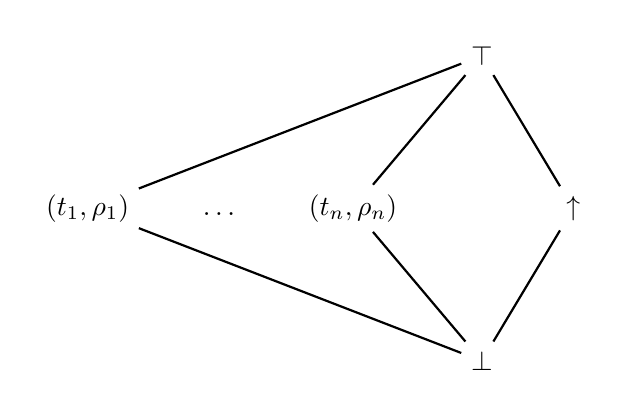
\begin{tikzpicture}
     \matrix (m) [matrix of math nodes, row sep=4em, column sep=2em]
    {              &        &             & \top &       \\
      (t_1,\rho_1) & \ldots & (t_n,\rho_n) &      & \fail \\
                   &        &             & \bot &       \\
    };

    \draw [thick] (m-2-1) -- (m-1-4);
    \draw [thick] (m-2-3) -- (m-1-4);
    \draw [thick] (m-2-5) -- (m-1-4);
    \draw [thick] (m-3-4) -- (m-2-1);
    \draw [thick] (m-3-4) -- (m-2-3);
    \draw [thick] (m-3-4) -- (m-2-5);
    \end{tikzpicture}
  \]

  We next define the category $\Naive$ where objects are elements of $N$, arrows are tuples $(x,y) : x \rightarrow y$ for $(x,y) \in N \times N$, the identity $\id_x = (x,x)$, and  composition $(y,z) \circ (x,y) = (x,z).$ Additionally we define the unary operation \emph{reverse} and binary operations \emph{meet} and \emph{join} on arrows with \[(x,y)^{-1} \coloneqq (y,x),\] \[ (x_1,x_2) \sqcup (y_1,y_2) \coloneqq (x_1 \sqcup x_2, y_1 \sqcup y_2) \] and \[ (x_1,x_2) \sqcap (y_1,y_2) \coloneqq (x_1 \sqcap x_2, y_1 \sqcap y_2), \] respectively.
\end{definition}

\begin{definition}\normalfont
  We continue by defining the abstraction functor $\alpha : \Rel(\State) \rightarrow \Naive$, for objects $S \subseteq \State$ by
  \[
     \alpha(S) \coloneqq \lub S
  \]
  and arrows $R : A \rightarrow B \subseteq \State \times \State$ by
  \[
     \alpha(R) \coloneqq (\lub A, \lub B).
  \]

  We now show, that $\alpha$ preserves identities and composition. For all $S \subseteq \State$, \begin{dmath*}\alpha(\id_S) = (\lub S, \lub S) = \id_{\lub S} = \id_{\alpha(S)}\end{dmath*} and for all $R : A \rightarrow B, S : B \rightarrow C \subseteq \State \times \State$, \begin{dmath*} \alpha(S \circ R) = (\lub A, \lub C) = (\lub B, \lub C) \circ (\lub B, \lub C) = \alpha(S) \circ \alpha(R). \end{dmath*}

  Furthermore, we show that $\alpha$ preserves reverse and all binary meet and joins. Given any arrows $R: X_1 \rightarrow X_2$ and $S:Y_1 \rightarrow Y_2$, since $R^{-1} : X_2 \rightarrow X_1,$
  \begin{dmath*}
    \alpha(R^{-1}) = (\lub X_2, \lub X_1)
                   = (\lub X_1, \lub X_2)^{-1}
                   = \alpha(R)^{-1}.
  \end{dmath*}
  Observe that $R \cup S : X_1 \cup Y_1 \rightarrow X_2 \cup Y_2$ and since $N$ is a complete partial order, it holds that $\forall A,B. \lub(A \cup B) = (\lub A) \sqcup (\lub B),$ then
 \begin{dmath*} \alpha(R \cup S) = (\lub(X_1 \cup Y_1),\lub(X_2\cup Y_2))
                                 = ((\lub X_1) \sqcup (\lub Y_1), (\lub X_2) \sqcup (\lub Y_2))
                                 = (\lub X_1,\lub X_2) \sqcup (\lub Y_1, \lub Y_2)
                                 = \alpha(R) \sqcup \alpha(S).
 \end{dmath*}
 Analoguosly for meets.
\end{definition}

\end{document}

%%% Local Variables:
%%% mode: latex
%%% TeX-master: t
%%% End:
